\section{Example Architecture and Scenario}
\label{section-architectureandscenario}

\begin{table}[t]
\begin{threeparttable}
{\footnotesize
\begin{tabularx}{\textwidth}{clrlXr}

\multicolumn{1}{c}{\textbf{\large{Type}}} &
\multicolumn{1}{c}{\textbf{\large{Name}}} &
\multicolumn{2}{c}{\textbf{\large{Power (mW)}}} &
\multicolumn{1}{c}{\textbf{\large{Performance}}} &
\multicolumn{1}{c}{\textbf{\large{ID}}}
\\ \toprule 

\multirow{6}{*}{\vspace{-0.15in}\textbf{CPU}} &
\multirow{2}{*}{ARM Cortex-M4\tnote{11}~\cite{cortexm4-web}} &
0.9\tnote{1} & &
75 MHz, 94 MIPS\tnote{2} &
\multirow{2}{*}{\textbf{P1}}
\\

& & &
15.6 &
300 MHz, 375 MIPS
&
\\ \cmidrule(l){2-6}

& \multirow{2}{*}{ARM Cortex-R4\tnote{11}~\cite{cortexr4-web}} &
4.6\tnote{1} & &
206 MHz, 342 DMIPS\tnote{2} &
\multirow{2}{*}{\textbf{P2}}
\\

& & &
78.8 &
620 MHz, 1030 DMIPS
&
\\ \cmidrule(l){2-6}

& \multirow{2}{*}{ARM Cortex-A9~\cite{cortexa9-web}} &
23.5\tnote{1} & &
415 MHz, 1037 DMIPS\tnote{2} &
\multirow{2}{*}{\textbf{P3}}
\\

& & &
400 &
830 MHz, 2075 DMIPS
&
\\ \toprule

\multirow{8}{*}{\vspace*{-0.15in}\textbf{Memory}} &
\multirow{2}{*}{\textbf{32~MB} ISSI SDRAM~\cite{issi32MBsdram-datasheet}} &
81 & &
Refresh only &
\multirow{2}{*}{\textbf{M1}}
\\

& & &
108 &
166 MHz
&
\\ \cmidrule(l){2-6}

&
\multirow{2}{*}{\textbf{256~MB} Micron ``Slow'' DDR2} &
239\tnote{10} & &
Refresh only &
\multirow{2}{*}{\textbf{M2}}
\\

& & &
405 &
266 MHz, 478Mtps
&
\\ \cmidrule(l){2-6}

&
\multirow{2}{*}{\textbf{1~GB} Micron ``Slow'' DDR2} &
322\tnote{10} & &
Refresh only &
\multirow{2}{*}{\textbf{M3}}
\\

& & &
482 &
266 MHz, 478Mtps
&
\\ \cmidrule(l){2-6}

%&
%\multirow{2}{*}{\textbf{2~GB} Micron ``Slow'' DDR2} &
%337 & &
%Refresh only &
%\multirow{2}{*}{\textbf{M4}}
%\\
%
%& & &
%582 &
%266 MHz, 478Mtps
%&
%\\ \cmidrule(l){2-6}
%
%&
%\multirow{2}{*}{\textbf{256~MB} Micron ``Fast'' DDR2} &
%346 & &
%Refresh only &
%\multirow{2}{*}{\textbf{M5}}
%\\
%
%& & &
%549 &
%400 Mhz, 720Mtps
%&
%\\ \cmidrule(l){2-6}

&
\multirow{2}{*}{\textbf{1~GB} Micron ``Fast'' DDR2} &
559\tnote{10} & &
Refresh only &
\multirow{2}{*}{\textbf{M4}}
\\

& & &
835 &
400 Mhz, 720Mtps
&
\\ \toprule

\multirow{6}{*}{\vspace*{-0.15in}\textbf{Storage}} &
\multirow{2}{*}{\textbf{2~GB} MicroSD Card} &
20\tnote{5} & &
Idle &
\multirow{2}{*}{\textbf{S1}}
\\

& & &
100\tnote{5} &
25 MBps\tnote{6}
&
\\ \cmidrule(l){2-6}


& \multirow{2}{*}{\textbf{64~GB} OCZ SSD} &
200\tnote{7} & &
Idle &
\multirow{2}{*}{\textbf{S2}}
\\

& & &
1000\tnote{7} &
5.5 MBps\tnote{7}
&
\\ \cmidrule(l){2-6}

& \multirow{2}{*}{\textbf{320~GB} Seagate HDD} &
700\tnote{7} & &
Idle &
\multirow{2}{*}{\textbf{S3}}
\\

& & &
1800\tnote{7} &
1.6 MBps\tnote{7}
&
\\ \toprule

\multirow{6}{*}{\vspace{-0.15in}\textbf{Radio}} &
\multirow{2}{*}{\textbf{250~kbps}} TI CC2540 BLE & 
6.63\tnote{2} & &
10\% duty cycle\tnote{9} &
\multirow{2}{*}{\textbf{R1}}
\\

& & &
66.3\tnote{3} &
Receive mode\tnote{3}
& \\ \cmidrule(l){2-6}

&
\multirow{2}{*}{\textbf{179.2~kbps} EDGE 3G} &
10\tnote{8} & &
Idle &
\multirow{2}{*}{\textbf{R2}}
\\

& & &
1320\tnote{8} &
Transmit mode
& \\ \cmidrule(l){2-6}

&
\multirow{2}{*}{\textbf{11~Mbps} Marvell 88W8686 802.11bg} &
30.9\tnote{2} & &
10\% duty cycle\tnote{9} &
\multirow{2}{*}{\textbf{R3}}
\\

& & &
309.3\tnote{4} &
Idle mode\tnote{4}
& \\ \toprule

\end{tabularx}
}
{\footnotesize
\begin{tablenotes}
\item [1] Optimistic estimate based on an optimistic estimate of DVFS providing 1:5 performance and
1:17 power scaling\cite{jssc02-PowerPC-SoC}.
\item [2] Estimated based on scaled full-power performance.
\item [3] Receive-only in high-sensitivity mode. Transmit numbers are not
significantly higher.
\item [4] Transmit and receive modes have very different power
consumption so usage is workload-dependent.
\item [5] Estimated due to lack of publicly-available datasheets.
\item [6] Maximum achievable.
\item [7] Measured by Tom's Hardware~\cite{ssd-tomshardware} using a realistic read-write mixture workload.
\item [8] Estimated numbers based on 2008
whitepaper~\cite{option3gpower-whitepaper}.
\item [9] Duty cycling allows the receiver to save power by shifting energy
consumption to the sender, which has to remain online (as in 802.11
PSM) or send longer packets (as in 802.15.4 Low-Power
Listening~\cite{tinyos-lpl}).
\item [10] Estimated based on Micron leakage numbers.
\item [11] Capable of running a subset of the full instruction set architecture
used by P3.
\end{tablenotes}
}
\caption{\textbf{Performance and power consumption of various hardware
components.} We assume voltage gating can reduce the power draw of a disabled
component to near zero~\cite{islped-vdd-gate}.}
\end{threeparttable}
\label{table-components}
\end{table}


To motivate the need for power-agile computing, we provide an example. First,
we present a selection of components and demonstrate the tradeoffs inherent
in each class --- processors, memory, storage, and radios. Second, we
construct a hardware architecture consisting of two components from each
class and show that it can operate in many possible configurations drawing
orders-of-magnitude different amounts of power. Third, we illustrate the kind
of power-agile adaptation this proposal aims to study, showing how a device
might respond to fluctuating demand and availability. The example motivates
the research questions listed in Section~\ref{section-researchquestions}.

Because we are targeting mobile applications and environmentally-powered
microservers, we surveyed a selection of components appropriate for this
class of device. We assume it will require a processor, memory, stable
storage, and radio. Table~\ref{table-components} summarizes the performance
and power draw of thirteen different parts in these four classes.

The relationship between power and performance is complex and varies both
between and within each component class. The power consumption of a computing
device under the smallest load is directly proportional to the number of
powered transistors. Current 32- and 64-bit microprocessors incorporate as
few as 40,000 and as many as \textit{one billion} transistors. Similar
dynamics drive the variations in power consumption and performance found
in other system components.

Processors provide a smooth performance transition over a restricted power
envelope using DVFS, but cannot scale to zero due to leakage current that
increases as a function of the number of transistors. Memory chips have a
refresh cost that scales somewhat with their size and an addition scaling
component corresponding to usage. Storage devices differ based on whether
they include spinning components: those that do not (Flash-based) scale power
roughly with usage but at presently limited in their size. Today, very high
capacity drives still use spinning platters and suffer from the high
background power draw necessary to rotate them. Radios exhibit even more
interesting power-performance variation because usage depends both on
properties of the hardware and characteristics of the protocol. 3G radios
leverage the powered infrastructure to reduce their receiving costs but pay a
high overhead to communicate with distant base stations. 802.11 radios can
enter power-saving mode (PSM) which leverages base station infrastructure to
save client power. Bluetooth and 802.15.4 protocols have limited range but
much lower power consumption balanced between both ends of the link.

When compiling the numbers in Table~\ref{table-components} we ran up against
the limited amount of available data reflecting component power consumption
under realistic assumptions. Datasheets often omit this information, numbers
in press releases are difficult to believe, and much of the
publicly-available information is provided by hobbyist sites such as Tom's
Hardware~\cite{tomshardware-www}. \textbf{We have completed the table using
estimates based on our experience in this area.} \uline{As an appropriate
response to the lack of this important information, we propose to develop
useful workloads and measure component numbers and disseminate these results
to the research community.}

\begin{figure*}[t]
\centering
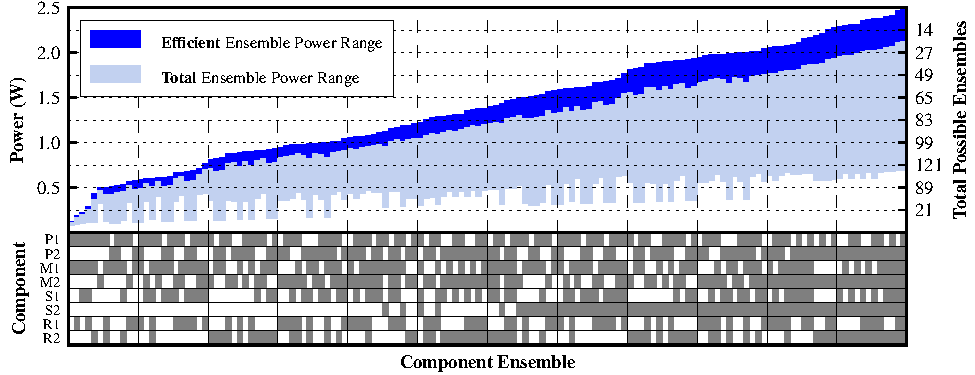
\includegraphics{./figures/componentgraph.pdf}

\caption{\textbf{Power envelopes of all 144 2x2x2x2 device component
ensembles.} Ensembles are sorted by increasing maximum power draw. The bottom
portion of the graph shows which components are active in each ensemble. The
top graph displays the power envelope for each ensemble, with the top 80\% of
the envelope --- the efficient operating range --- drawn in dark blue. The
numbers on the right axis indicate the number of possible ensembles that
might draw that much power: for example, there are 121 ensembles that could
consume 0.75~W, depending on the workload and how components are used.}
\vspace{-0.05in}
\label{figure-componentgraph}
\end{figure*}

Throughout the rest of the proposal we refer to a \textit{component ensemble}
as the set of components active at a given time, constraining the possible
ensembles to consist of (a) at least one or multiple processors and memory
chips and (b) zero, one or multiple storage devices or radios\footnote{While
many low-power processors come with small amounts of integrated memory, we
have conservatively chosen to require 32~MB of RAM in order to run embedded
versions of Linux. It is conceivable that our candidate device could enter an
active sleep state with a micro-kernel capable of fitting in the processor's
onboard RAM.}. Using the components presented in
Table~\ref{table-components}, we consider a potential 2x2x2x2 architecture
consisting of two components from each category --- \textbf{P1} and
\textbf{P3} (processors); \textbf{M1} and \textbf{M3} (memory); \textbf{S1}
and \textbf{S2} (storage); \textbf{R1} and \textbf{R3} (radios). We selected
these components to allow the overall architecture to operate across a wide
power range. It its lowest-power ensemble (P1,M1), the device has a 75~MHz
CPU and 32~MB of RAM, draws as little as 82~mW\footnote{We recognize that the
actual power consumption of a device integrating these components would be
higher due to power consumed by system buses, memory controllers, and other
essential components of a complete architecture.} and is roughly-equivalent
to a embedded sensor node; in its highest-power ensemble with all components
powered and active the device has multiple cores, over 1~GB of RAM, over
320~GB of storage, and Wifi and Bluetooth. Consuming almost 2500~mW of power,
it is similar to emerging high-end smartphones.

In total our device can activate \textit{144 possible component ensembles}.
Figure~\ref{figure-componentgraph} shows all possibilities and the power
range associated with each, and illustrates several key observations.
\textbf{First, there is wide variation in the power usage of component
ensembles even in an architecture with only two components per class.}
Incorporating more components per class would result in even more variation.
\textbf{Second, at any overall power level there are many components
ensembles that the device can use.} A diverse set of ensembles is available
at most power points: a fast processor, small memory chip, and slow disk; a
slow processor, large memory, and a fast radio; etc. Of course, not all
possible ensembles at a given power point may be possible or make sense --- a
processor of sufficient speed may be required to drive a high-bandwidth radio
--- but, given careful component choices, we think many will. It also may not
make sense to operate a component ensemble at a power level insufficiently to
allow high levels of component activity, but given the variations in load and
availability and the potential overhead of transitions between component
ensembles we believe that devices will spend some time at the low end of
ensemble power envelopes.

\begin{figure*}[t]
\centering
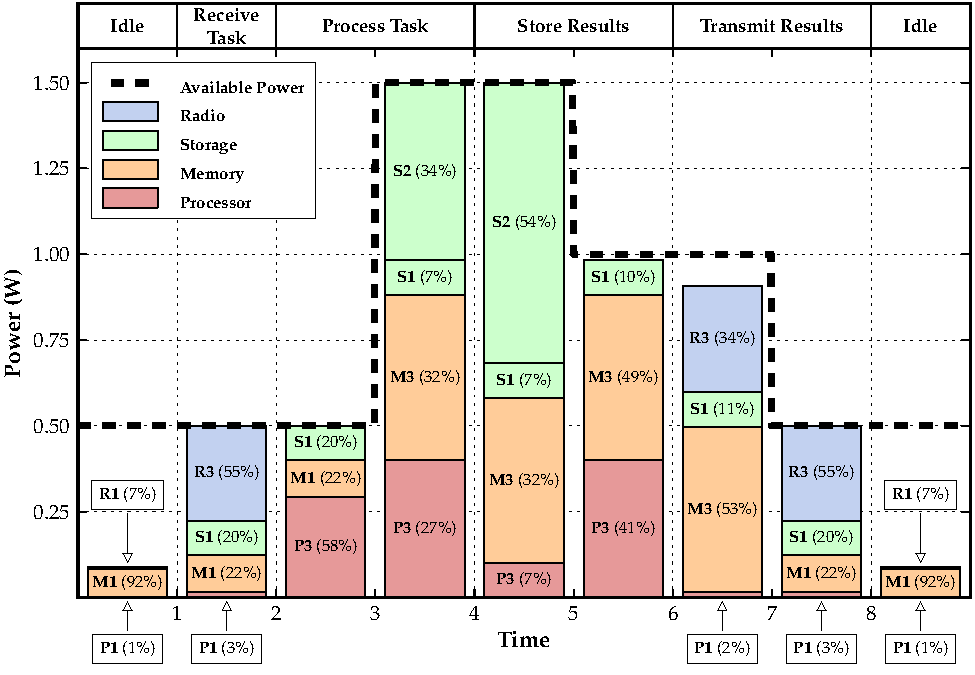
\includegraphics{./figures/transitiongraph.pdf}

\caption{\textbf{Device transitioning between component ensembles as power
availability and demand change.} This figure is described in more detail in
Section~\ref{section-motivatingexample}. Percentages shown are what the
component is contributing to the total ensemble power draw.}

\label{figure-transitiongraph}
\end{figure*}

We illustrate how our heterogeneous device might react to fluctuating power
availability and demand by transitioning between component ensembles in
Figure~\ref{figure-transitiongraph}. Imagine a wind-powered microserver made
available to mobile devices for task processing. Walking through the
scenario:

\begin{timeenum}

\item With no tasks to process, the device is in a low-power state with
\textbf{P1} and \textbf{M1} idle. Radio \textbf{R1} remains active at low
duty cycle awaiting incoming tasks. Unused power is being stored.

\item Alerted to an incoming task, the device activates high-power radio
\textbf{R3} to rapidly receive task data and low-power Flash storage
\textbf{S1} to store it. With 0.5~W of input power the device's power usage
is now matching availability.

\item After receiving task data, the device begins processing the task,
reconfiguring energy usage by activating the high-power processor \textbf{P3}
and disabling the radio \textbf{R3}.

\item With power availability suddenly increasing to 1.5~W and the device
still processing the task, it accelerates task processing by (a) activating
the larger, faster memory chip \textbf{M3} and (b) mirroring some storage
operations to the faster disk \textbf{S2}.

\item As the device begins storing results to disk, power usage shifts
towards I/O even as the device continues using the same component ensemble.

\item While it continues to store results, power availability suddenly drops
to 1~W. Unable to operate the fast disk \textbf{S2}, the device shifts to
storing all results on \textbf{S1}. To reduce space on the smaller disk, it
compresses data on the fly, resulting in higher usage of processor
\textbf{P3}.

\item Ready to return results, radio \textbf{R3} is activated, and the device
switches to processor \textbf{P1} which is sufficient to move results from
disk \textbf{S1} to the radio.

\item When power availability falls again, the device
disables \textbf{M3} and switches to the smaller memory chip \textbf{M1}.

\item Once task results have been offloaded, the device returns to its
low-power idle state.

\end{timeenum}

Examining this scenario yields additional insights. \textbf{First, ensemble
transitions can be the result of changing availability (t = 3, t = 7), demand
(t = 2, t = 6) or both.} Thus, power-agility is crucial even for systems
designed to operate on a static power budget, perhaps tuned to match the
efficient region of a voltage regulator. \textbf{Second, heterogeneous
architectures can be used to shift available power towards the components of
the system most useful for completing a given task.} At t = 2, the system is
able to shift power from the radio to the CPU as demand shifts from
communication to processing. \textbf{Finally, when availability and demand
are fluctuating, the operating system can help prepare for necessary ensemble
transitions.} Depending on the layout and status of pages in M3 at t = 7,
transitioning to M1 may be easy or it may be difficult.
